\chapter{Dinamica dei Robot}
Questo capitolo si occupa di scrivere le equazioni del moto di un robot manipolatore a catena aperta semplice facendo uso delle equazioni di Lagrange. Scrivere le equazioni del moto vuol dire esprimere le azioni degli attuatori che fanno muovere il meccanismo in funzione di
\begin{equation}
	\underline{q}, \; \dot{\underline{q}}, \; \ddot{\underline{q}}, \; \underline{\gamma}
\end{equation}
con $\underline{q}$ coordinate lagrangiane e $\underline{\gamma}$ eventuali azioni che il meccanismo esercita sull'ambiente esterno, come spostare un peso con l'organo terminale.

Un obiettivo rilevante dello studio della dinamica dei robot è quello della progettazione degli algoritmi di controllo che si basano sulla conoscenza delle forze agli attuatori ricavati dal modello dinamico.
\paragraph{}
Scrivere le equazioni del moto di un meccanismo vuol dire esplicitare la \emph{funzione di dinamica inversa},
\begin{equation}
	\underline{\tau} = \underline{\tau}(\underline{q}, \underline{\dot{q}}, \underline{\ddot{q}}, \underline{\gamma})
\end{equation}
dove $\underline{\tau}$ è il vettore delle azioni che gli attuatori esercitano sui giunti (forze o coppie).


Il modello dinamico può essere facilmente invertito ricavando la \emph{funzione di dinamica diretta},
\begin{equation}
	\underline{\ddot{q}} = \underline{\ddot{q}}(\underline{q}, \underline{\dot{q}}, \underline{\tau}, \underline{\gamma}).
\end{equation} 

\subsubsection{Tecniche:}
Esistono due metodi per ricavare le equazioni del moto,
\begin{enumerate}
	\item La \textbf{formulazione di Lagrange}: si basa sulle equazioni di Lagrange ricavate nelle \emph{Appendici}, ha l'enorme vantaggio di essere \emph{sistematica}, fornisce le equazioni del moto in forma analitica e compatta che evidenzia la matrice di inerzia, matrice delle forze centrifughe e di Coriolis e il vettore delle forze gravitazionale. Utile per progettare un sistema di controllo.
	\item La \textbf{formulazione di Newton-Eulero}: è intrinsecamente un metodo ricorsivo che risulta efficace da un punto di vista computazionale, infatti sfrutta la natura seriale a catena aperta tipica del manipolatore. Questo metodo non viene trattato in queste dispense.
\end{enumerate}

\subsubsection{Dinamica diretta e inversa:}
Vediamo le sostanziali differenze tra le due,
\begin{itemize}
	\item La \textbf{Dinamica diretta} consiste nel determinare, le accelerazioni risultanti ai giunti $\ddot{\underline{q}}$, assegnate $\underline{\tau}$ ed eventualmente $\underline{\gamma}$ e note le posizioni $\underline{q}$ e le velocità $\dot{\underline{q}}$ dei giunti.
	\item La \textbf{Dinamica inversa} consiste nel determinare le azioni degli attuatori $\underline{\tau}$ necessarie alla generazione del movimento specificato assegnando le accelerazioni, velocità e posizioni dei giunti e note le eventuali forze all'organo terminale $\underline{\gamma}$.
\end{itemize}

Al livello computazionale, per un manipolatore a $n$ giunti, il numero di operazioni richieste dal calcolo della dinamica risulta pari a $O(n^2)$ per la dinamica diretta e $O(n)$ per la dinamica inversa. 

\section{Formulazione di Lagrange}
Con la \emph{formulazione di Lagrange}, le equazioni del moto possono essere ricavate con un approccio indipendente dal sistema di coordinate di riferimento. Scelto un insieme di variabili $q_i$ per $i = 1, \cdots, n$, denominate \emph{coordinate lagrangiane o generalizzate} che descrivono le posizioni degli elementi meccanici costituenti il manipolatore a $n$ gradi di libertà, si definisce \emph{lagrangiana} del sistema meccanico la funzione
\begin{equation}
	\mathcal{L}(\underline{\dot{q}}, \underline{q}, t) = T(\underline{\dot{q}}, \underline{q}, t) - U(\underline{q}, t)
\end{equation} 
in cui $T$ ed $U$ sono le rispettivamente l'energia cinetica e l'energia potenziale totali del sistema.

La scelta delle coordinate lagrangiane non è unica ma, per i robot a catena aperta che trattiamo, è ovvio scegliere come coordinate lagrangiane gli elementi del vettore $\underline{q}$ delle coordinate dei giunti, si tratta quindi di rotazioni $\theta_i$ o traslazioni $d_i$.

\paragraph{}
Notiamo che tra le coordinate lagrangiane di un robot con base fissa che si muove liberamente nello spazio non esistono vincoli al livello differenziale, ovvero tra le derivate temporali di $\underline{q}$, pertanto sono sistemi meccanici con vincoli \emph{olonomi}, o in breve, \emph{sistemi olonomi}. Pertanto possiamo scrivere le $n$ equazioni di Lagrange,
\begin{equation}
	\frac{d}{dt} \Biggl( \frac{\partial \mathcal{L}}{\partial \dot{q}_i} \Biggr) - \frac{\partial \mathcal{L}}{\partial q_i} = Q_i \qquad \forall i = 1, \cdots, n
\end{equation}
dove $Q_i$ indica la componente lagrangiana delle forze attive \emph{non conservative} lungo la direzione della coordinata lagrangiana $q_i$. Bisogna puntualizzare però, che riferendoci ad un robot, le forze non conservative $Q_i$ sono composto in linea del tutto generale da:
\begin{itemize}
	\item \emph{Forza che gli attuatori esercitano sul giunto} $i$: Ovvero, $\underline{\tau}_{\,i}$
	\item \emph{Forza di attrito agente sul giunto} $i$: ovvero, $\underline{\tau}_{\,i,f}$
	\item \emph{Effetti delle forze esterne sul giunto} $i$: ovvero, $-J_i^T \underline{\gamma}$
\end{itemize}
pertanto, il secondo membro della $8.5$, in del tutto generale assume la forma 
\begin{equation*}
	Q_i = \underline{\tau}_{\,i}-\underline{\tau}_{\,i,f} - J_i^T \underline{\gamma}
\end{equation*}

Le $n$ equazioni in $(8.5)$ rappresentano le \emph{equazioni del moto} del manipolatore.

\subsection{Motoriduttore con pendolo in gravità}
Per capire meglio questo metodo, facciamo un esempio e applichiamo il metodo delle equazioni di Lagrange ad un pendolo, mobile nel piano verticale, azionato da un motoriduttore. La procedura è semplice,
\begin{enumerate}
	\item Calcoliamo l'energia cinetica del sistema $T$.
	\item Calcoliamo l'energia potenziale del sistema $U$.
	\item Calcoliamo la Lagrangiana $\mathcal{L} = T-U$.
	\item Infine, deriviamo la Lagrangiana secondo la $(8.5)$ e otteniamo le equazioni del moto.
\end{enumerate} 
il pendolo di massa $m$ giace sul piano $xy$ e possiede tensore di inerzia baricentrico $I_l$ e un tensore di inerzia del motoriduttore pari a $I_m$. 
\begin{center}
	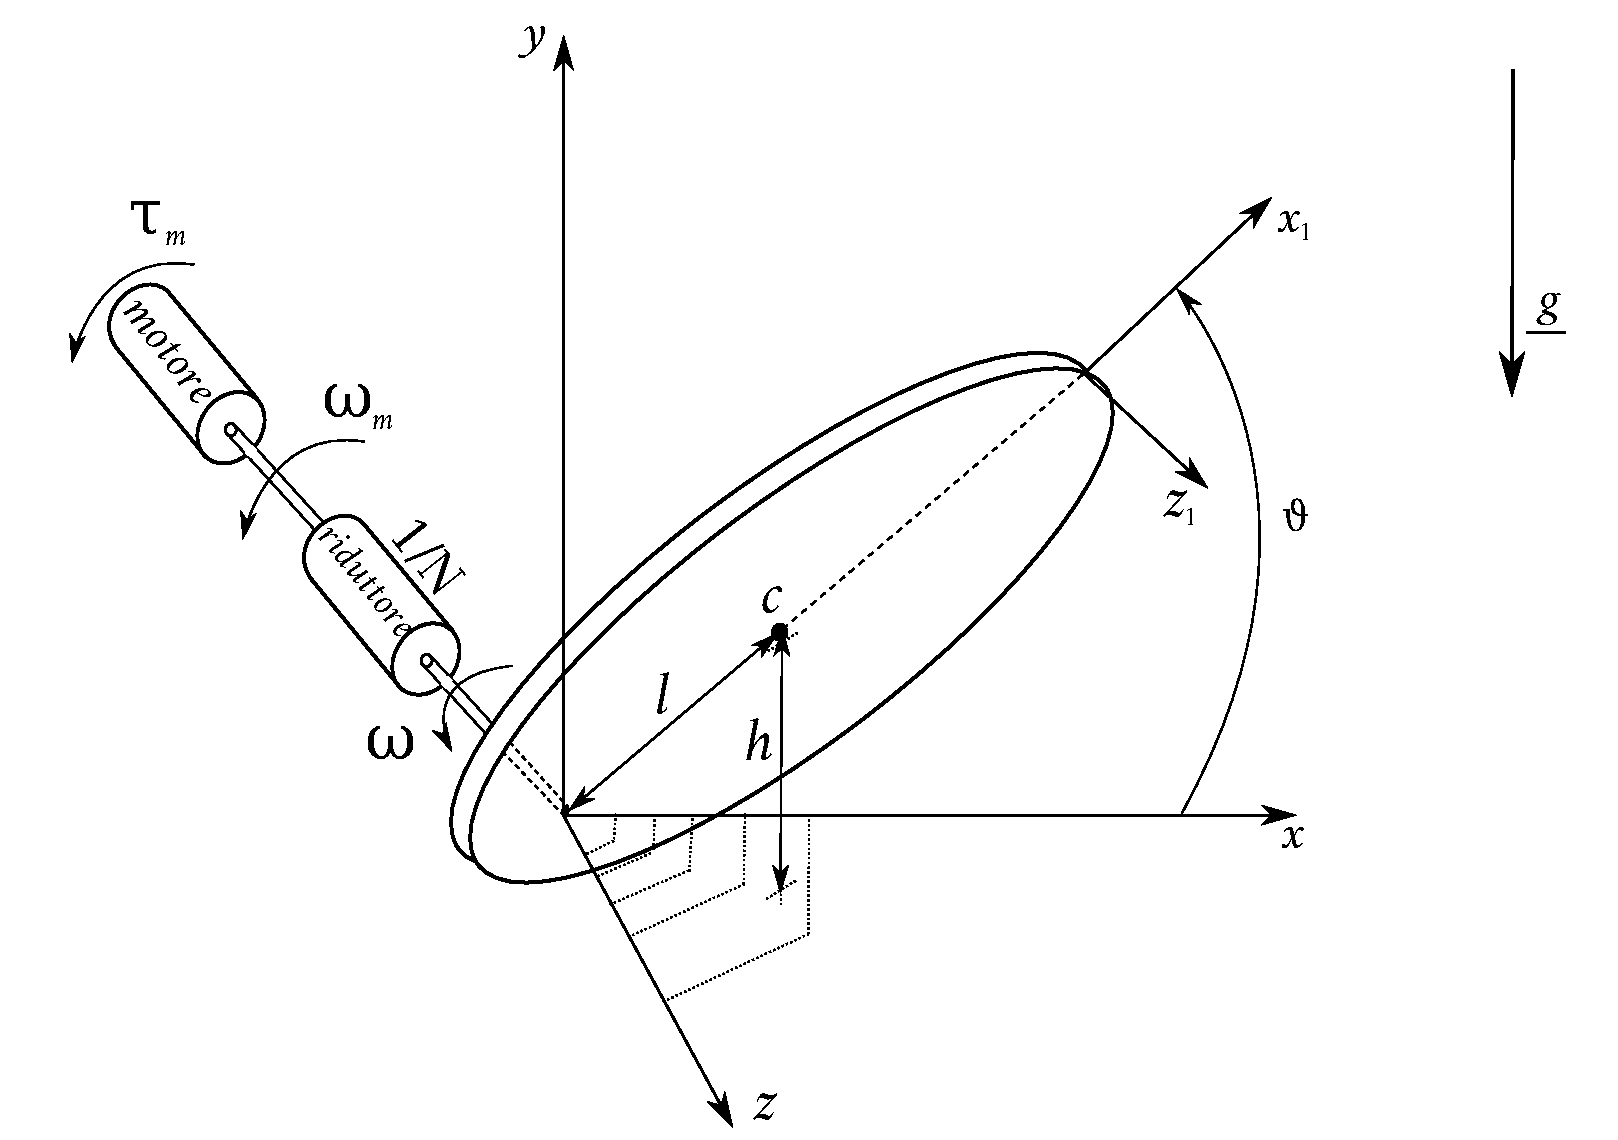
\includegraphics[scale=0.4]{pendolo.pdf}
	\caption{Pendolo motorizzato in gravità.}
\end{center}

Supponendo che il rapporto di riduzione sia $1/N$ otteniamo, 
\begin{equation}
	\begin{cases}
		\omega_m = N\omega = \dot{\vartheta}_m = N \dot{\vartheta} \\
		\tau_m \dot{\vartheta}_m = \tau \dot{\vartheta} \; \rightarrow \; \tau = \tau_m \frac{\dot{\vartheta}_m}{\dot{\vartheta}} = N \tau_m
	\end{cases}
\end{equation}
dove con $\tau$ indichiamo le forze non conservative, e pertanto scriviamo
\begin{equation*}
	\underline{\omega}_{\,l} = 
	\begin{bmatrix}
		0 \\ 0 \\ \dot{\vartheta}
	\end{bmatrix}
	\qquad I_l = 
	\begin{bmatrix}
		I_{xx} & -I_{xy} & -I_{xz} \\
		-I_{xy} & I_{yy} & -I_{yz} \\
		-I_{xz} & -I_{yz} & I_{zz} \\
	\end{bmatrix}
	\qquad \underline{p}_{\,c} =
	\begin{bmatrix}
		l \cos(\vartheta) \\ 
		l \sin(\vartheta) \\
		p_{cz} \\
	\end{bmatrix} 
	\qquad \dot{\underline{p}_{\,c}} = 
	\begin{bmatrix}
		-l \sin(\vartheta) \\
		l \cos(\vartheta) \\
		0 \\
	\end{bmatrix}
\end{equation*}
con $\underline{p}_{\,c}$ vettore identificativo del baricentro nella terna di riferimento e $p_{cz}$ costante.

\subsubsection{1. Calcoliamo l'energia cinetica del sistema:}
\paragraph{}
Per calcolare l'energia cinetica complessiva, sommiamo quella del motoriduttore $T_m$ con quella del link $T_l$. Iniziamo con la prima,
\begin{equation}
	T_m = \frac{1}{2} I_m \dot{\vartheta}_m^2 = \frac{1}{2}I_m N^2 \dot{\vartheta}^2
\end{equation}

per $T_l$ consideriamo la $(C.34)$, ovvero, il moto di traslazione del centro di massa a cui si somma una rotazione attorno al centro di massa e otteniamo,
\begin{equation}
	T_l = \frac{1}{2} m \dot{\underline{p}}_{\,c}^T \dot{\underline{p}}_{\,c} + \frac{1}{2} \underline{\omega}_{\,l}^T I_l \underline{\omega}_{\,l}
\end{equation}
e quindi, l'energia cinetica del sistema complessivo $T = T_m + T_l$ è
\begin{equation*}
	T = \frac{1}{2} \Biggl( N^2 I_m \dot{\vartheta}^2 + 
	\begin{bmatrix}
		0 & 0 & \dot{\vartheta}
	\end{bmatrix}
	\cdot
	\begin{bmatrix}
		I_{xx} & -I_{xy} & -I_{xz} \\
		-I_{xy} & I_{yy} & -I_{yz} \\
		-I_{xz} & -I_{yz} & I_{zz} \\
	\end{bmatrix}
	\cdot
	\begin{bmatrix}
		0 \\
		0 \\
		\dot{\vartheta} \\
	\end{bmatrix}
	+ m l^2
	\begin{bmatrix}
		-\sin(\vartheta) & 
		\cos(\vartheta) &
		0
	\end{bmatrix}
	\begin{bmatrix}
		- \sin(\vartheta) \\
		\cos(\theta) \\
		0 \\
	\end{bmatrix}
	\dot{\vartheta}^2
	\Biggr)
\end{equation*}
e quindi, otteniamo
\begin{equation}
	T = \frac{1}{2}\underbrace{(N^2 I_m + I_{zz} + ml^2)}_{I} \dot{\vartheta}^2 = \frac{1}{2} I \dot{\vartheta}^2
\end{equation}
dove con $I$ indichiamo il momento di inerzia totale del sistema, ridotto all'asse $z$ del pendolo.
\subsubsection{2. Calcoliamo l'energia potenziale del sistema:}
\paragraph{}
L'energia potenziale di un corpo rigido soggetto all'accelerazione di gravità $\underline{g}$, vale $U = mgh$, dove $m$ è la massa del corpo, $g$ è il modulo dell'accelerazione di gravità e $h$ è la quota del baricentro rispetto al riferimento scelto come zero per l'energia potenziale. Noi scegliamo la quota dell'origine $O$ come zero per l'energia potenziale, ovvero il piano $xz$.

Anche in questo caso dovremmo fare lo stesso discorso dell'energia cinetica, ovvero dovremmo avere $U = U_l + U_m$ ma l'energia potenziale $U_m$ è nulla per la scelta dello zero per l'energia potenziale. Otteniamo quindi
\begin{equation}
	U = mg\underbrace{l \sin(\vartheta)}_{h}
\end{equation}

\subsubsection{3. Calcoliamo la lagrangiana:}
La lagrangiana $\mathcal{L} = T - U$, scegliendo $\vartheta$ come coordinata generalizzata, risulta,
\begin{equation}
	\mathcal{L} = \frac{1}{2} I \dot{\vartheta}^2 - mgl \sin(\vartheta)
\end{equation}

\subsubsection{4. Equazioni del moto:}
Per calcolarci le equazioni del moto, ovvero la componente delle forze attive non conservative $Q = N \tau_m$, eseguiamo le derivate,
\begin{eqnarray}
	\frac{d}{dt} \Biggl( \frac{\partial \mathcal{L}}{\partial \dot{\vartheta}} \Biggr) = \frac{d}{dt} \Biggl( I\dot{\vartheta} \Biggr) = I \ddot{\vartheta} \\
	\frac{\partial \mathcal{L}}{\partial \vartheta} = -mg l \cos(\vartheta)
\end{eqnarray}
e otteniamo
\begin{equation}
	\frac{d}{dt} \Biggl( \frac{\partial \mathcal{L}}{\partial \dot{\vartheta}} \Biggr) - \frac{\partial \mathcal{L}}{\partial \vartheta} = I \ddot{\vartheta} + mgl \cos(\vartheta) = N\tau_m = Q
\end{equation}

\section{Metodo sistematico Lagrangiano}
Adesso, vogliamo applicare la \emph{formulazione di Lagrange} ad un robot a $n$ giunti, e chiaramente procederemo come nell'esempio del pendolo, esplicitando l'energia cinetica, l'energia potenziale e infine le equazioni del moto. 

\subsection{Energia cinetica}
Consideriamo un manipolatore con $n$ bracci rigidi, l'energia cinetica totale è data dalla somma dei contributi relativi al moto di ogni braccio e dei contributi relativi al moto degli attuatori ai giunti:
\begin{equation}
	T = \sum_{i = 1} ^{n} (T_{l_i} + T_{m_i})
\end{equation} 
in cui $T_{l_i}$ denota l'energia cinetica del braccio $i$ e $T_{m_i}$ denota l'energia cinetica del motore che aziona il giunto $i$.

\subsubsection{$\bullet$ Energia cinetica dei $link$:}
Facciamo l'ipotesi semplificatrice che ogni giunto $i$ rotoidale o prismatico, sia attuato da un singolo motoriduttore con statore solidale al link $i-1$. Quindi, il link $i$ collega il giunto $i$ al giunto $i+1$ e ad esso vi sarà attaccato anche il motore che muove il giunto $i+1$ con statore $i+1$ solidale al link $i$. Con riferimento alla figura,
\begin{center}
	\includegraphics[scale=0.40]{caratterizzazioneCinematica.pdf}
	\caption{Caratterizzazione cinematica del braccio $i$ ai fini della formulazione di Lagrange.}
\end{center}
definiamo,
\begin{itemize}
	\item $\underline{p}_{\,l_i} := $ vettore posizione del centro di massa del corpo rigido formato dal $link_i + statore_{i+1}$.
	\item $\dot{\underline{p}_{\,l_i}} := $ velocità del centro di massa.
	\item $\underline{\omega}_{\,i} := $ velocità angolare del $link_i$.
	\item $\underline{p}_{\,i}^* := $ punto generico appartenente al volume del $link$.
	\item $\underline{r}_{\,i} := $ vettore posizione del generico punto $\underline{p}_{\,i}^*$ rispetto a $\underline{p}_{\,l_i}$.
	\item $z_i$ e $z_{i+1}$ sono gli assi rispettivamente del giunto $i$ e del giunto $i+1$.
\end{itemize}

\paragraph{}
L'energia cinetica della particella di massa $\rho dV$ risulta
\begin{equation}
	dT = \frac{1}{2} \dot{\underline{p}}_{\,i}^{*^T}  \dot{\underline{p}}_{\,i}^* \rho dV
\end{equation}
pertanto, l'energia cinetica del braccio $i$ risulta
\begin{equation}
	T_{l_i} = \frac{1}{2} \int_{V_{l_i}} \dot{\underline{p}}_{\,i}^{*^T}  \dot{\underline{p}}_{\,i}^* \rho dV
\end{equation}
con $V_{l_i}$ il volume del braccio $i$. Considerando il vettore posizione $\underline{p}_{\,i}^*$ della particella elementare e il vettore posizione $\underline{p}_{\,l_i}$ del baricentro del braccio, entrambi riferiti alla terna base si ha
\begin{equation}
	\underline{r}_{\, i} = 
	\begin{bmatrix}
		r_x & r_y & r_z
	\end{bmatrix}^T 	
	= \underline{p}_{\,i}^* - \underline{p}_{\,l_i}
\end{equation}
con 
\begin{equation}
	\underline{p}_{\,l_i} = \frac{1}{\int_{V_{l_i}}\rho dV} \int_{V_{l_i}} \underline{p}_{\,i}^* \rho dV
\end{equation}
dove $\int_{V_{l_i}}\rho dV = m_{l_i}$ è la massa del braccio. A questo punto esprimiamo $\underline{p}_{\,i}^*$ applicando la formula fondamentale dei moti rigidi,
\begin{equation}
	\underline{p}_{\,i}^* = \dot{\underline{p}_{\,l_i}} + \underline{\omega}_{\,i} \times \underline{r}_{\,i} = \dot{\underline{p}_{\,l_i}} + S(\underline{\omega}_{\,i})\underline{r}_{\,i}
\end{equation}
e inoltre, si ha
\begin{align*}
	\underline{p}_{\,i}^{*^T} \underline{p}_{\,i}^* = \Bigl( \dot{\underline{p}}_{\,l_i}^T + \underline{r}_{\,i}^T S^T(\underline{\omega}_{\,i})\Bigr) \Bigl(\dot{\underline{p}}_{\,l_i} + S(\underline{\omega}_{\,i})\underline{r}_{\,i} \Bigr) =\\
	= \dot{\underline{p}}_{\,l_i}^T \underline{\dot{p}}_{\,l_i} + 2\dot{\underline{p}}_{\,l_i}^T S(\underline{\omega}_{\,i}) \underline{r}_{\,i} + \underbrace{\underline{r}_{\,i}^T S^T(\underline{\omega}_{\,i})S(\underline{\omega}_{\,i}) \underline{r}_{\,i}}_{\underline{\omega}_{\,i}^T S^T(\underline{r}_{\,i})S(\underline{r}_{\,i})\underline{\omega}_{\,i}}
\end{align*}
dove $\underline{\omega}_{\,i}$ indica la velocità angolare del braccio.

Riscrivendo la $(8.17)$ considerando la $(8.20)$ otteniamo,
\begin{align*}
	T_{l_i} = \int_{V_{l_i}} dT = \frac{1}{2} \int_{V_{l_i}} \Bigl[ \underline{\dot{p}}_{\,l_i}^T \underline{\dot{p}}_{\,l_i} + \underline{\omega}_{\,i}^T S^T(\underline{r}_{\,i}) S(\underline{r}_{\,i})\underline{\omega}_{\,i} + 2 \dot{\underline{p}}_{\,l_i}^T S(\underline{\omega}_{\,i})\underline{r}_{\,i} \Bigr] \rho dV = \\
	= \underbrace{\frac{1}{2} \underline{\dot{p}}_{\,l_i}^T \underline{\dot{p}}_{\,l_i} \int_{V_{l_i}} \rho dV}_{traslazione} + \underbrace{\frac{1}{2} \underline{\omega}_{\,i}^T \Biggl[ \int_{V_{l_i}} S^T(\underline{r}_{\,i})S(\underline{r}_{\,i}) \rho dV \Biggr] \underline{\omega}_{\,i}}_{rotazione} + \underbrace{\frac{1}{2} 2 \underline{\dot{p}}_{\,l_i}^T S(\underline{\omega}_{\,i}) \int_{V_{l_i}} \underline{r}_{\,i} \, \rho dV}_{= 0}
\end{align*}
e adesso analizziamo il termine di rotazione, 
\begin{align*}
	\int_{V_{l_i}} S^T(\underline{r}_{\,i})S(\underline{r}_{\,i}) \rho dV = 
	\int_{V_{l_i}}
	\underbrace{
	\begin{bmatrix}
		0 & r_z & -r_y \\
		-r_z & 0 & r_x \\
		r_y & -r_x & 0 \\
	\end{bmatrix}
	}_{S^T(\underline{r}_{\,i})}
	\cdot
	\underbrace{
	\begin{bmatrix}
		0 & -r_z & r_y \\
		r_z & 0 & -r_x \\
		-r_y & r_x & 0 \\
	\end{bmatrix}
	}_{S(\underline{r}_i)}
	\rho dV
\end{align*}
e portando l'integrale dentro la matrice otteniamo,
\begin{equation}
	\begin{bmatrix}
		\int_{V_{l_i}} (r_y^2 + r_z^2) & \int_{V_{l_i}} - r_x r_y & \int_{V_{l_i}} -r_x r_z \\
		\int_{V_{l_i}} -r_x r_y & \int_{V_{l_i}} (r_x^2 + r_z^2) & \int_{V_{l_i}} -r_y r_z \\
		\int_{V_{l_i}} -r_x r_z & \int_{V_{l_i}} -r_y r_z & \int_{V_{l_i}} (r_x^2 + r_y^2) \\
	\end{bmatrix}
	= I_{l_i}
\end{equation}
ovvero, $I_{l_i}$ è il \emph{tensore di inerzia} del link $i$ relativo al suo baricentro espresso in terna base. Notiamo che se la terna solidale al braccio $i$ coincide con la terna centrale di inerzia, i momenti centrifughi sono nulli e il tensore diventa una matrice diagonale.

Quindi, l'energia cinetica relativa al link $i$ è
\begin{equation}
	T_{l_i} = \underbrace{\frac{1}{2} m_{l_i} \underline{\dot{p}}_{\,l_i}^T \underline{\dot{p}}_{\,l_i}}_{traslazione} + \underbrace{\frac{1}{2} \underline{\omega}_{\,i}^T I_{l_i} \underline{\omega}_{\,i}}_{rotazione}
\end{equation}

\paragraph{}
Per scrivere le equazioni di Lagrange, visto che è una meccanica scalare, dobbiamo trovare un'espressione in cui siano esplicitate le coordinate generalizzate (quindi le coordinate di giunto) $\underline{q}$ e $\dot{\underline{q}}$. Pertanto, per esprimere la $(8.22)$, associamo a $\dot{\underline{p}}_{\,l_i}$ uno Jacobiano di traslazione $J_P^{(l_i)} \in \mathbb{R}^{3 \times n}$ e associamo a $\underline{\omega}_{\,i}$ uno Jacobiano di rotazione $J_O^{(l_i)} \in \mathbb{R}^{3 \times n}$, quindi otteniamo
\begin{equation}
	\begin{cases}
		\dot{\underline{p}}_{\,l_i} = J_P^{(l_i)} \underline{\dot{q}} = J_{P1}^{(l_i)} \dot{q}_1 + \cdots + J_{Pi}^{(l_i)} \dot{q}_i \\
		\underline{\omega}_{\,i} = J_O^{(l_i)} \underline{\dot{q}} = J_{O1}^{(l_i)} \dot{q}_1 + \cdots + J_{Oi}^{(l_i)} \dot{q}_i \\
	\end{cases}
\end{equation}
vengono evidenziati i contributi delle colonne degli Jacobiani relativi alle velocità dei giunti che precedono il braccio $i$ in esame, quindi gli Jacobiani da considerare sono, 
\begin{align}
	J_P^{(l_i)} = 
	\begin{bmatrix}
		J_{P1}^{(l_i)} & \cdots & J_{Pi}^{(l_i)} & 0 & \cdots & 0
	\end{bmatrix} \\
	J_O^{(l_i)} = 
	\begin{bmatrix}
		J_{O1}^{(l_i)} & \cdots & J_{Oi}^{(l_i)} & 0 & \cdots & 0
	\end{bmatrix} 
\end{align} 
e possiamo calcolare questi elementi per $j \leq i$ come segue,
\begin{align}
	J_{Pj}^{(l_i)} =
	\begin{cases}
		\underline{k}_{j-1} \qquad\qquad \qquad\qquad \text{prismatico} \\
		\underline{k}_{j-1} \times (\underline{p}_{\,l_i} - \underline{O}_{\,j-1}) \qquad \text{rotoidale}
	\end{cases}\\
	J_{Oj}^{(l_i)} = 
	\begin{cases}
		0 \qquad\qquad  \text{prismatico} \\
		\underline{k}_{j-1} \qquad\qquad \text{rotoidale}
	\end{cases}
\end{align}
dove $\underline{O}_{\,j-1}$ è il vettore posizione dell'origine e $k_{\,j-1}$ è il versore dell'asse $z$ della terna $j-1$.

Pertanto, riscrivendo l'energia cinetica del braccio $i$ della $(8.22)$ risulta
\begin{equation}
	T_{l_i} = \frac{1}{2} \underline{\dot{q}}^T \Biggl[ m_{l_i} J_P^{(l_i)^T} J_P^{(l_i)} + J_O^{(l_i)^T} I_{l_i} J_O^{(l_i)} \Biggr]\underline{\dot{q}}
\end{equation}

\subsubsection{$\bullet$ Energia cinetica dei motori:}
Per calcolare il contributo di energia cinetica relativo al motore del giunto $i$, si procede in maniera analoga a quanto visto prima. Considerando il caso tipico di motori elettrici rotanti che possono azionare sia giunti rotoidali che prismatici e supponiamo che il contributo dello statore è incluso in quello relativo al braccio su cui tale motore è situato e quindi calcoliamo solo il contributo del rotore.

\begin{center}
	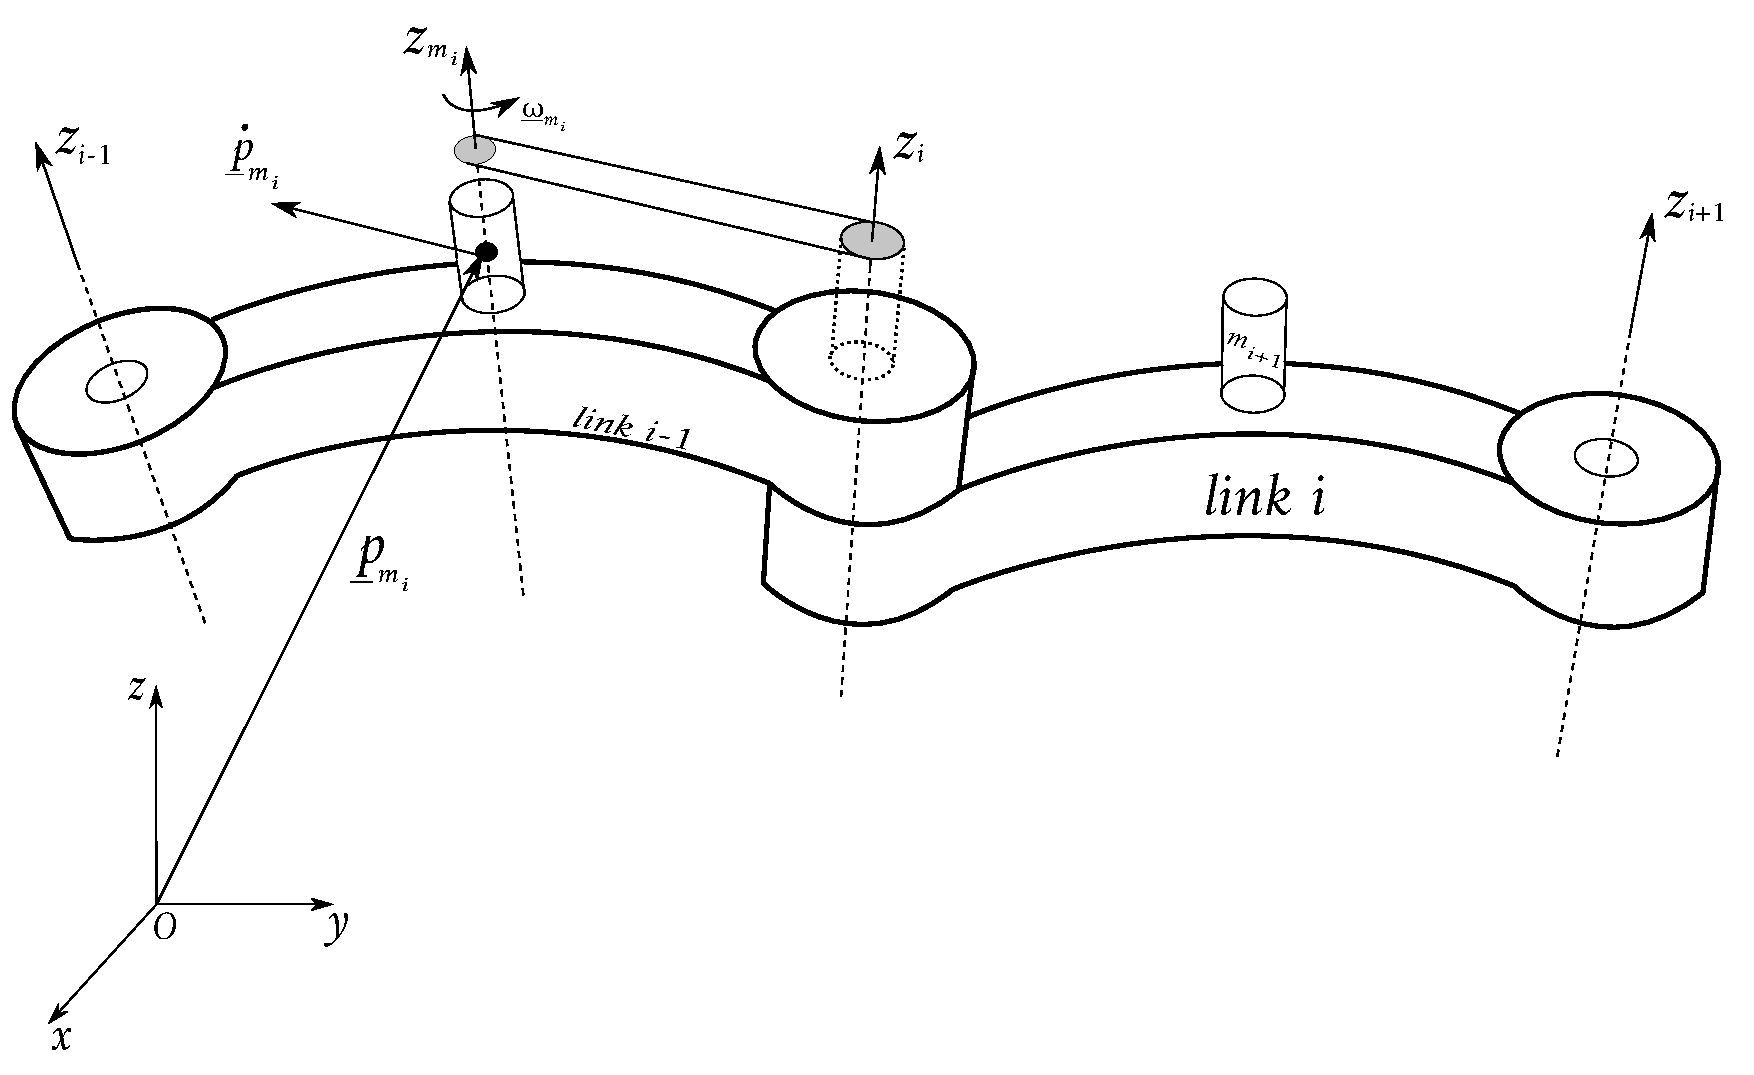
\includegraphics[scale=0.43]{caratterizzazioneMotore.pdf}
	\caption{Caratterizzazione cinematica del motore $i$ posto nel link $i-1$.}
\end{center}

Il motore del giunto $i$ si ritiene collocato sul braccio $i-1$, si suppone che non vi siano moti indotti, ovvero il motore del giunto non aziona il moto di altri giunti e pertanto la matrice di trasmissione è diagonale. L'energia cinetica del rotore $i$ può scriversi come
\begin{equation}
	T_{m_i} = \frac{1}{2} m_{m_i} \dot{\underline{p}}_{\,m_i}^T \dot{\underline{p}}_{\,m_i} + \frac{1}{2} \underline{\omega}_{\,m_i}^T I_{m_i} \underline{\omega}_{\,m_i}
\end{equation}
con $m_{m_i}$ massa del rotore, $\underline{\dot{p}}_{\,m_i}$ velocità lineare del baricentro del rotore, $I_{m_i}$ tensore di inerzia del rotore relativo al baricentro, e $\underline{\omega}_{\,m_i}$ velocità angolare del rotore. 

Notiamo inoltre che se il rapporto di riduzione tra giunto $i$ (prismatico o rotoidale) e il motoriduttore è $1/N_i$, allora otteniamo,
\begin{equation}
	\dot{\vartheta}_i = N_i \dot{\vartheta}_{m_i} \qquad \dot{d}_i = N_i \dot{\vartheta}_{m_i}
\end{equation} 
con $\vartheta_{m_i}$ posizione angolare del rotore.

\paragraph{}
L'energia cinetica $T_{m_i}$ del rotore $i$ appena trovata deve essere espressa attraverso le coordinate generalizzate, per fare ciò, procediamo in maniera analoga all'energia cinetica dei link. Infatti, associamo
\begin{equation}
	\begin{cases}
		\dot{\underline{p}}_{\,m_i} = J_P^{(m_i)} \underline{\dot{q}} \\
		\underline{\omega}_{\,m_i} = J_O^{(m_i)} \underline{\dot{q}}
	\end{cases}
\end{equation}
con $J_P^{(m_i)}$ Jacobiano di traslazione del motore e $J_O^{(m_i)}$ jacobiano di orientazione del motore, così definiti
\begin{align}
	J_P^{(m_i)} = 
	\begin{bmatrix}
		J_{P,1}^{(m_i)} & \cdots & J_{P,i-1}^{(m_i)} & 0 & \cdots & 0
	\end{bmatrix} \\
	J_O^{(m_i)} = 
	\begin{bmatrix}
		J_{O,1}^{(m_i)} & \cdots & J_{O,i-1}^{(m_i)} & 0 & \cdots & 0
	\end{bmatrix} 
\end{align}
e notiamo che $J_{Pi}^{m_i} = 0$ perchè il baricentro del rotore è posizionato sull'asse di rotazione del rotore. Calcoliamo gli elementi delle matrici,
\begin{align}
	J_{Pj}^{(m_i)} =
	\begin{cases}
		\underline{k}_{j-1} \qquad\qquad \qquad\qquad \text{prismatico} \\
		\underline{k}_{j-1} \times (\underline{p}_{\,m_i} - \underline{O}_{\,j-1}) \qquad \text{rotoidale}
	\end{cases}\\
	J_{Oj}^{(m_i)} = 
	\begin{cases}
		J_{Oj}^{(l_i)} \qquad\qquad  j = 1,\cdots,i-1 \\
		k_i z_{m_i} \qquad\qquad j = i
	\end{cases}
\end{align}
con $k_i$ rapporto di trasmissione meccanica (come può essere $1/N_i$), $z_{m_i}$ versore dell'asse di rotazione del rotore, $J_{Oj}^{(l_i)}$ Jacobiano di orientazione del link $i$ e $\underline{O}_{\,j-1}$ vettore posizione dell'origine della terna relativa al giunto $j-1$.

\paragraph{}
Quindi la $(8.29)$ si riscrive,
\begin{equation}
	T_{m_i} = \frac{1}{2} \underline{\dot{q}} \Biggl[ m_{m_i} J_P^{(m_i)^T} J_P^{(m_i)} + J_O^{(m_i)^T} I_{m_i} J_O^{(m_i)} \Biggr]\underline{\dot{q}}
\end{equation}

\subparagraph{Nota sui tensori:}
I tensori $I_{l_i}$ e $I_{m_i}$ della $(8.28)$ e della $(8.36)$ si possono scrivere usando i tensori visti rispetto alla terna solidale al link $l_i$ e motore $m_i$,
\begin{equation}
	I_{l_i} = R_i I_{l_i}^i R_i^T \qquad I_{m_i} = R_i I_{m_i}^i R_i^T
\end{equation}
con $R_i$ matrice di rotazione dalla terna solidale al braccio $i$ alla terna base, pertanto i tensori $I_{l_i}$ e $I_{m_i}$ sono tensori visti dalla terna base.

\subsubsection{$\bullet$ Energia cinetica totale:}
Andiamo a scrivere la $(8.15)$ usando la $(8.28)$ e $8.36$,
\begin{equation}
	T = \frac{1}{2} \underline{\dot{q}}^T \sum_{i = 1}^n \underbrace{\Biggl[ m_{l_i} J_P^{(l_i)^T} J_P^{(l_i)} + J_O^{(l_i)^T} I_{l_i} J_O^{(l_i)} + m_{m_i} J_P^{(m_i)^T} J_P^{(m_i)} + J_O^{(m_i)^T} I_{m_i} J_O^{(m_i)} \Biggr]}_{B(\underline{q})} \underline{\dot{q}}
\end{equation}
il termine nelle parentesi quadre rappresenta la \emph{matrice di inerzia} $B(\underline{q}) \in \mathbb{R}^{n \times n}$ che risulta \emph{simmetrica}, \emph{definita positiva} e \emph{dipendente dalla configurazione in generale}.

\subsection{Energia potenziale}
Per l'energia potenziale, il discorso è analogo a quanto visto per l'energia cinetica. Ovvero, l'energia potenziale totale del sistema è data dalla somma dei contributi relativi ad ogni braccio e dei contributi relativi ai rotori dei motori dei giunti,
\begin{equation}
	U = \sum_{i=1}^n (U_{l_i} + U_{m_i})
\end{equation}

Per il contributo del link, utilizziamo la figura 8.2 e otteniamo,
\begin{equation}
	U_{l_i} = - \int_{V_{l_i}} \underline{g}^T \underline{p}_{\,i}^* \rho dV = -m_{l_i} \underline{g}^T \underline{p}_{\,l_i}
\end{equation}
in cui $\underline{g}$ è il vettore accelerazione gravitazionale riferito alla terna base.

Per quanto riguarda il contributo del rotore $i$, con riferimento alla figura 8.3 si ha,
\begin{equation}
	U_{m_i} = - m_{m_i} \underline{g}^T \underline{p}_{\,m_i}
\end{equation}

Pertanto, riscrivendo la $(8.39)$ otteniamo,
\begin{equation}
	U = - \sum_{i=1}^n \Bigl( m_{l_i} \underline{g}^T \underline{p}_{\,l_i} + m_{m_i} \underline{g}^T \underline{p}_{\,m_i} \Bigr)
\end{equation}
e notiamo che è una funzione solo di $\underline{q}$ e non di $\underline{\dot{q}}$ perchè dipende dai vettori $\underline{p}_{\,l_i}$ e $\underline{p}_{\,m_i}$. 

\subsection{Equazioni del moto}
Tenendo conto delle espressioni $(8.38)$ e $(8.42)$ andiamo a scrivere la Lagrangiana,
\begin{equation}
	\mathcal{L}(\underline{q}, \dot{\underline{q}}) = T(\underline{q}, \dot{\underline{q}}) - U(\underline{q})
\end{equation}
a questo punto, eseguendo le varie derivate, otteniamo
\begin{equation}
	B(\underline{q})\ddot{\underline{q}} + n(\underline{q}, \underline{\dot{q}}) = \underline{Q}
\end{equation}
dove $\underline{Q}$ rappresenta il vettore delle forze attive non conservative e $n(\underline{q}, \underline{\dot{q}})$ ha la seguente forma
\begin{equation}
	n(\underline{q}, \underline{\dot{q}}) = \dot{B}(\underline{q})\dot{\underline{q}} - \frac{1}{2} \Biggl( \frac{\partial}{\partial \underline{q}} \Bigl( \dot{\underline{q}}^T B(\underline{q}) \dot{\underline{q}} \Bigr) \Biggr)^T + \Biggl( \frac{\partial U(\underline{q})}{\partial \underline{q}} \Biggr)^T 
\end{equation}
\paragraph{}
Per esplicitare le forze non conservative che compiono lavoro sui giunti del manipolatore, andiamo a definire le seguenti componenti:
\begin{itemize}
	\item \textbf{Le forze di attuazione:} rappresentate dal vettore $\underline{\tau} \in \mathbb{R}^n$.
	\item \textbf{Le forze di attrito viscoso:} $F_v \underline{\dot{q}}$ con $F_v \in \mathbb{R}^{n \times n}$ matrice dei coefficienti di attrito viscoso.
	\item \textbf{Le forze di attrito statico:} $f_s(\underline{q}, \underline{\dot{q}})$ che possiamo esplicitare come attrito \emph{coulumbiano} $f_s = F_s\, sgn(\underline{\dot{q}})$ con $F_s \in \mathbb{R}^{n \times n}$ e $sgn(\underline{\dot{q}}) \in \mathbb{R}^{n \times 1}$ le cui componenti sono date dalle funzioni segno delle velocità dei singoli giunti.
	\item \textbf{Le forze di contatto:} definite solo se l'organo terminale è in contatto con l'ambiente, allora vi è un \emph{wrench} di forza pari a $J^T(\underline{q})\underline{\gamma}$ con $\underline{\gamma}$ vettore di forza e momento esercitati dall'organo terminale del manipolatore sull'ambiente.  
\end{itemize}
e otteniamo
\begin{equation}
	\underline{Q} = \underline{\tau} - F_v \, \underline{\dot{q}} - F_s\, sgn(\underline{\dot{q}}) - J^T(\underline{q})\underline{\gamma}
\end{equation}

\paragraph{}
Le equazioni del moto $(8.44)$ possono essere riscritte nella forma matriciale compatta che rappresenta il \emph{modello dinamico nello spazio dei giunti},
\begin{equation}
	B(\underline{q})\ddot{\underline{q}} + C(\underline{q}, \underline{\dot{q}}) \underline{\dot{q}} + \underline{g}(\underline{q}) = \underline{\tau} - F_v \,\underline{\dot{q}} - F_s \, sgn(\underline{\dot{q}}) - J^T(\underline{q}) \underline{\gamma}
\end{equation}
dove:
\begin{itemize}
	\item $B(\underline{q}) \in \mathbb{R}^{n \times n}$ è la \emph{matrice di inerzia}.
	\item $C(\underline{q}, \underline{\dot{q}}) \in \mathbb{R}^{n \times n}$ è la matrice dei termini di Coriolis e centrifughi.
	\item $\underline{g}(\underline{q}) \in \mathbb{R}^n$ è il vettore delle azioni delle forze di gravità sui giunti. Si ricava nel derivare l'energia potenziale totale, $\partial U / \partial q_i = g_i(\underline{q})$.
\end{itemize}
e infine, come abbiamo già accennato, possiamo ricavare la \emph{dinamica diretta},
\begin{equation}
	\underline{\ddot{q}} = B^{-1}(\underline{q}) \Bigl[ \underline{\tau} - C(\underline{q}, \underline{\dot{q}})\underline{\dot{q}} - F_v \,\underline{\dot{q}} - F_s \, sgn(\underline{\dot{q}}) - \underline{g}(\underline{q}) - J^T(\underline{q}) \underline{\gamma} \Bigr]
\end{equation}
dove chiaramente abbiamo invertito la matrice $B(\underline{q})$, operazione possibile dato che la matrice è simmetrica e definita positiva.

\section{Proprietà del modello dinamico}
Presentiamo delle proprietà notevoli del modello dinamico ricavato nella $(8.47)$, un'importante proprietà che non approfondiamo ma che si utilizza per dimostrare la stabilità per certi algoritmi di controllo è l'anti-simmetria della matrice così definita
\begin{equation}
	N(\underline{q}, \underline{\dot{q}}) = \dot{B}(\underline{q}) - 2C(\underline{q}, \underline{\dot{q}})
\end{equation}
ovvero,
\begin{equation}
	\underline{v}^T \, N(\underline{q}, \underline{\dot{q}})\, \underline{v} = 0 \qquad \forall \underline{v} \in \mathbb{R}^{n \times 1}
\end{equation}
detto ciò, passiamo a proprietà più significative.

\subsection{Linearità dei parametri dinamici}
Una importante proprietà del modello dinamico è la \emph{linearità} rispetto ai \emph{parametri dinamici} caratteristici die bracci e dei rotori del manipolatore. L'obiettivo è quello di individuare questi parametri indipendenti dalla configurazione dei giunti del manipolatore, consideriamo pertanto il \emph{link} $l_i$ come corpo rigido che comprende il \emph{motore} $m_{i+1}$ come in figura
\begin{center}
	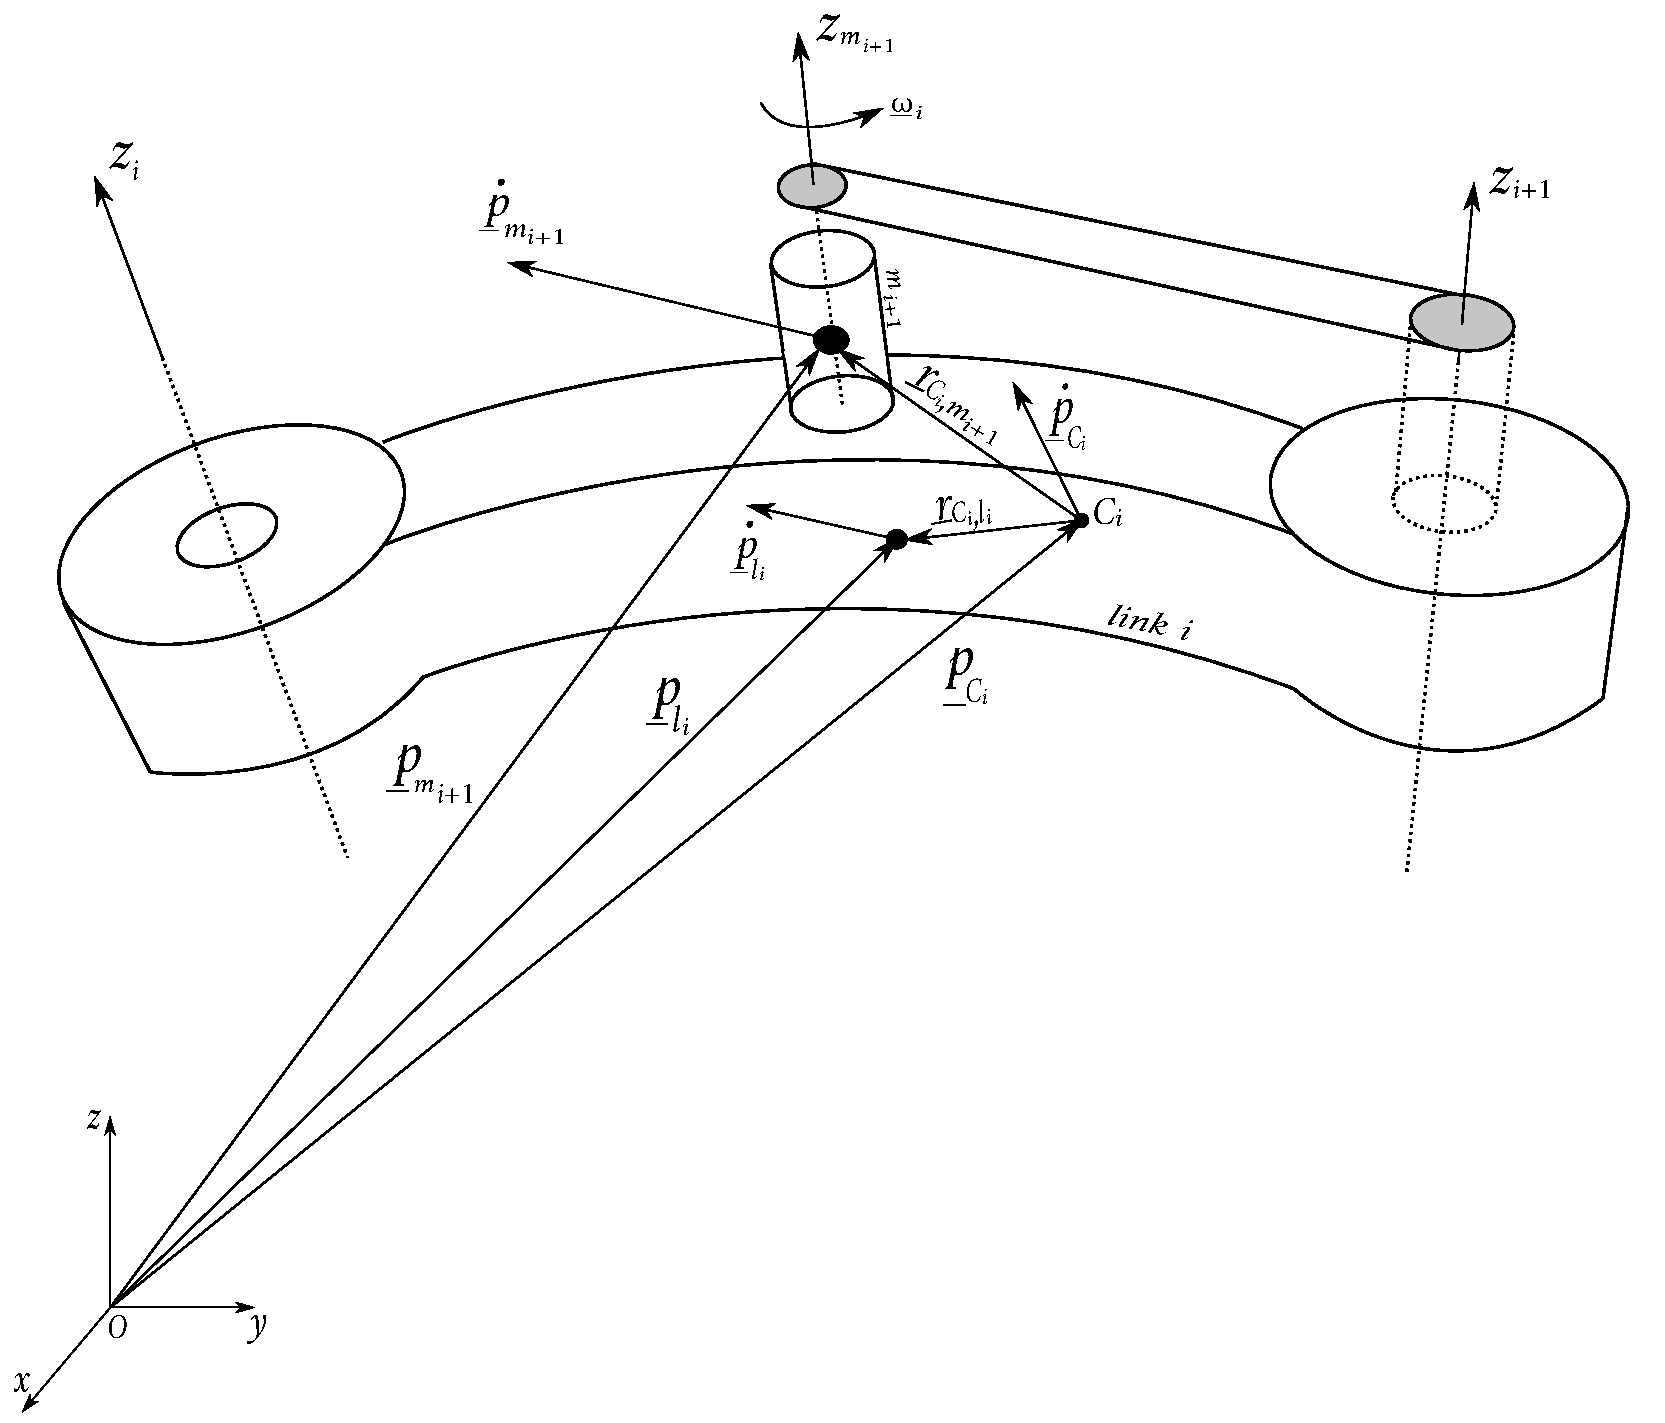
\includegraphics[scale=0.4]{linearitaProprietaDinamici.pdf}
	\caption{Caratterizzazione cinematica del \emph{link} $i$}
\end{center}
e pertanto possiamo definire il centro di massa di questo corpo rigido composto dal link e dal rotore come $C_i$, quindi utilizzando la descrizione cinematica dei rigidi otteniamo
\begin{equation}
	\begin{cases}
		\underline{r}_{\,C_i,l_i} = \underline{p}_{\,l_i} - \underline{p}_{\,C_i} \\
		\underline{r}_{\,C_i,m_{i+1}} = \underline{p}_{\,m_{i+1}} - \underline{p}_{\,C_i} 
	\end{cases}
	\qquad
	\begin{cases}
		\underline{\dot{p}}_{\,l_i} = \underline{\dot{p}}_{\,C_i} + \underline{\omega}_{\,i} \times \underline{r}_{\,C_i,l_i} \\
		\underline{\dot{p}}_{\,m_{i+1}} = \underline{\dot{p}}_{\,C_i} + \underline{\omega}_{\,i} \times \underline{r}_{\,C_i,m_{i+1}}
	\end{cases}
\end{equation}
dove $\underline{p}_{\,C_i}$ denota il vettore posizione del baricentro dell'insieme braccio + rotore.

\paragraph{}
Scriviamo l'energia cinetica del complessivo corpo rigido $i$, 
\begin{equation}
	T_i = T_{l_i} + T_{m_{i+1}}
\end{equation}
con $T_{l_i}$ pari a $(8.22)$ e $T_{m_{i+1}}$ pari a $(8.29)$ con la massa $m_{i+i}$ invece della massa $m$.

Per poter scrivere l'energia cinetica si riscrive $T_{l_i}$ e $T_{m_{i+1}}$ con le $(8.51)$ e otterremo, col teorema di Steiner, i seguenti tensori di inerzia relativi al baricentro complessivo $\underline{p}{\,C_i}$,
\begin{equation}
	\begin{cases}
		\overline{I}_{l_i} = I_{l_i} + m_{l_i} S^T(\underline{r}_{\,C_i, l_i})S(\underline{r}_{\,C_i, l_i}) \\
		\overline{I}_{m_{i+1}} = I_{m_{i+1}} + m_{m_{i+1}} S^T(\underline{r}_{\,C_i, m_{i+1}})S(\underline{r}_{\,C_i, m_{i+1}})
	\end{cases}
\end{equation}
e pertanto, esprimiamo la \emph{massa complessiva} del rigido $i$ come $m_i = m_{l_i} + m_{m_{i+1}}$ e il \emph{tensore di inerzia complessivo} come $\overline{I}_i = \overline{I}_{l_i} + \overline{I}_{m_{i+1}}$. 

\paragraph{}
Finora abbiamo espresso tutto in terna fissa, ma dato che l'obiettivo è trovare dei parametri indipendenti dalle configurazioni di giunto, andiamo ad esprimere le seguenti relazioni
\begin{equation}
	\begin{cases}
		\underline{p}_{\,C_i}^i = \underline{p}_i^i + \underline{r}_{\,i,C_i}^i \\
		\underline{\dot{p}}_{\,C_i}^i = \underline{\dot{p}}_i^i + \underline{\omega}_i^i \times \underline{r}_{\,i,C_i}^i
	\end{cases}
\end{equation}
in cui si sono espressi tutti i vettori nella terna $i$ e chiaramente $\underline{r}_{i,C_i}^i$ è fisso in tale terna e vale
\begin{equation}
	\underline{r}_{\,i,C_i}^i = 
	\begin{bmatrix}
		l_{C_ix} & l_{C_iy} & l_{C_iz}
	\end{bmatrix}^T
\end{equation}

Inoltre, il tensore di inerzia $I_{m_i}^{m_i}$ è chiaramente diagonale, otteniamo
\begin{equation}
	I_{m_{i+1}} \cdot z_{m_{i+1}} = I_{m_{i+1}zz} \cdot z_{m_{i+1}}
\end{equation}
dove, il membro di sinistra è il tensore e quello di destra è il momento di inerzia proiettato nel proprio asse di rotazione.

Riscrivendo l'energia cinetica otteniamo il tensore di inerzia rispetto all'origine della terna $i$ 
\begin{equation}
	\hat{I}_{i}^{i} = \overline{I}_{i}^i + m_i S^T(\underline{r}_{\,i, C_i}^i)S(\underline{r}_{\,i, C_i}^i)
\end{equation}
e il \emph{momento primo di inerzia}
\begin{equation}
	m_i \underline{r}_{\,i,C_i}^i = 
	\begin{bmatrix}
		m_i l_{C_ix} \\
		m_i l_{C_iy} \\
		m_i l_{C_iz} 
	\end{bmatrix}
\end{equation}
quindi scriviamo il tensore,
\begin{equation}
	\hat{I}_{i}^{i} = 
	\begin{bmatrix}
		\hat{I}_{ixx} & -\hat{I}_{ixy} & -\hat{I}_{ixz} \\
		-\hat{I}_{ixy} & \hat{I}_{iyy} & -\hat{I}_{iyz} \\
		-\hat{I}_{ixz} & -\hat{I}_{iyz} & \hat{I}_{izz}
	\end{bmatrix}
\end{equation}

Pertanto $T_i$ del corpo rigido braccio $i$ e rotore $i+1$ è lineare rispetto ai parametri dinamici seguenti:
\begin{itemize}
	\item la \emph{massa} $m_i = m_{l_i} + m_{m_{i+1}}$
	\item le tre componenti del \emph{momento primo di inerzia} $m_i \underline{r}_{\,i,C_i}^i$
	\item le sei componenti del tensore di inerzia $\hat{I}_i^i$ solidale al link
	\item il momento di inerzia del motore rispetto al proprio asse di rotazione $I_{m_izz}$
\end{itemize} 
\paragraph{}
L'energia potenziale dell'insieme braccio $i$ e rotore $i+1$ risulta
\begin{equation}
	U_i = -\underline{g}_i^T(m_i \underline{p}_i^i + m_i \underline{r}_{\,i,C_i}^i)
\end{equation}
e pertanto è lineare rispetto alla massa e alle tre componenti del momento primo di inerzia.

Quindi, infine possiamo scrivere la lagrangiana come
\begin{equation}
	\mathcal{L} = \sum_{i=1}^n \Bigl( \beta_{T_i} - \beta_{U_i} \Bigr) \underline{\pi_i}
\end{equation}
dove abbiamo evidenziato il vettore dei \emph{parametri dinamici},
\begin{equation}
	\underline{\pi_i} = 
	\begin{bmatrix}
		m_i \\ m_i l_{C_ix} \\ m_i l_{C_iy} \\ m_i l_{C_iz} \\ \hat{I}_{ixx} \\ \hat{I}_{ixy} \\ \hat{I}_{ixz} \\ \hat{I}_{iyy} \\ \hat{I}_{iyz} \\ \hat{I}_{izz} \\ I_{m_izz}
	\end{bmatrix}
	\in \mathbb{R}^{11 \times 1}
\end{equation}

I vettori $\beta_{T_i} \in \mathbb{R}_{11 \times 1}$ e $\beta_{U_i} \in \mathbb{R}_{11 \times 1}$ consentono di scrivere la lagrangiana in funzione di $\underline{\pi_i}$, inoltre anche le operazioni di derivazioni non alterano la proprietà di linearità. Pertanto la \emph{forza generalizzata} non conservativa del giunto $i$ può scriversi come
\begin{equation}
	Q_i = \sum_{j=1}^n y_{ij}^T \, \underline{\pi_j}
\end{equation}
dove 
\begin{equation}
	y_{ij} = \frac{d}{dt} \Biggl( \frac{\partial \beta_{T_j}}{\partial \dot{q}_i} \Biggr) - \frac{\partial \beta_{T_j}}{\partial q_i} + \frac{\partial \beta_{U_j}}{\partial q_i}
\end{equation}
e notiamo che le derivate parziali sono nulle per $j<i$, pertanto otteniamo la seguente espressione matriciale, esplicitando $Q_i = \tau_i$,
\begin{equation}
	\begin{bmatrix}
		\tau_1 \\
		\tau_2 \\
		\vdots \\
		\tau_n \\
	\end{bmatrix}
	= 
	\begin{bmatrix}
		y_{11}^T & y_{12}^T & \cdots & y_{1n}^T \\
		0^T & y_{22}^T & \cdots & y_{2n}^T \\
		\vdots & \vdots & \ddots & \vdots \\
		0^T & 0^T & \cdots & y_{nn}^T
	\end{bmatrix}
		\cdot
	\begin{bmatrix}
		\pi_1 \\
		\pi_2 \\
		\vdots \\
		\pi_n \\
	\end{bmatrix}
\end{equation}
e notiamo che questa espressione matriciale esprime la \textbf{linearità del modello dinamico} del manipolatore rispetto a un insieme opportuno di \textbf{parametri dinamici}.

Inoltre, è opportuno includere il coefficiente di attrito viscoso e di attrito Coulombiano tra i parametri di $\underline{\pi_i}$ arrivando a $13$ parametri per ogni giunto. Scrivendo in forma compatta,
\begin{equation}
	\underline{\tau} = Y(\underline{q}, \underline{\dot{q}}, \underline{\ddot{q}}) \underline{\pi}
\end{equation}
dove $\underline{\pi} \in \mathbb{R}^{p \times 1}$ è un vettore di $p$ parametri \emph{costanti}, con $p < 13n$ in quanto non è detto che tutti e 13 parametri di ogni giunto compaiano esplicitamente nella $(8.65)$; Si ha $Y \in \mathbb{R}^{n \times p}$ matrice che rispecchia la proprietà di linearità del modello dinamico dipendente dalle posizioni, velocità e accelerazioni dei giunti. $Y$ prende il nome di \emph{regressore}. 

\subsection{Identificazioni dei parametri dinamici}
Questa non è una proprietà vera e propria, ma riguarda il calcolo effettivo dei parametri dinamici della $(8.62)$. In effetti, il loro calcolo è parecchio laborioso anche se si usano software di calcolo.

Per ricavare stime accurate dei parametri dinamici si ricorre a tecniche di identificazione che sfruttano la proprietà di linearità $(8.65)$. Queste tecniche consentono di ricavare il vettore $\underline{\pi}$ sulla base di misure effettuate, durante l'esecuzione di opportune traiettorie di moto imposte al manipolatore, così da ricavare numericamente la matrice $Y$.

A questo punto, supponendo di aver ricavato, nell'esecuzione della traiettoria imposta al manipolatore, le misure di forza, posizioni, velocità e accelerazioni ai giunti in corrispondenza degli istanti di tempo $t_1, \cdots, t_N$, si può scrivere
\begin{equation}
	\overline{\underline{\tau}} = 
	\begin{bmatrix}
		\underline{\tau}(t_1) \\
		\vdots \\
		\underline{\tau}(t_N)
	\end{bmatrix}
	= 
	\begin{bmatrix}
		Y(t_1) \\
		\vdots \\
		Y(t_N)
	\end{bmatrix}
	\underline{\pi}
	= \overline{Y} \underline{\pi}
\end{equation}
con un numero di istanti molto alto, ovvero $Nn \gg p$.

Risolvendo la $(8.67)$ con una tecnica ai minimi quadrati, si ottiene la soluzione nella forma
\begin{equation}
	\underline{\pi} = \Bigl( \overline{Y}^{\,T} \overline{Y} \Bigr)^{-1}  \overline{Y}^{\,T} \overline{\underline{\tau}}
\end{equation}
dove $\Bigl( \overline{Y}^{\,T} \overline{Y} \Bigr)^{-1}  \overline{Y}^{\,T}$ è la matrice pseudo-inversa di sinistra di $\overline{Y}$.